\section{\fwname Architecture}
\label{sec:architecture}

Repeated agent refinement calls for an execution engine that can apply local state changes and run long evaluations at low cost. \fwname uses a file-centric architecture to support targeted edits and manages context on demand to preserve prompt-cache reuse across the session lifecycle.

\subsection{Evolution Efficiency: File-Centric Architecture}
\label{sec:file-centric}

In general-purpose harnesses with large built-in system prompts and specialized tool definitions, an optimizer may have to search and rewrite a substantial instruction space to make a small behavioral change. Such changes can also introduce conflicts with existing instructions.

\begin{figure*}[t]
  \centering
  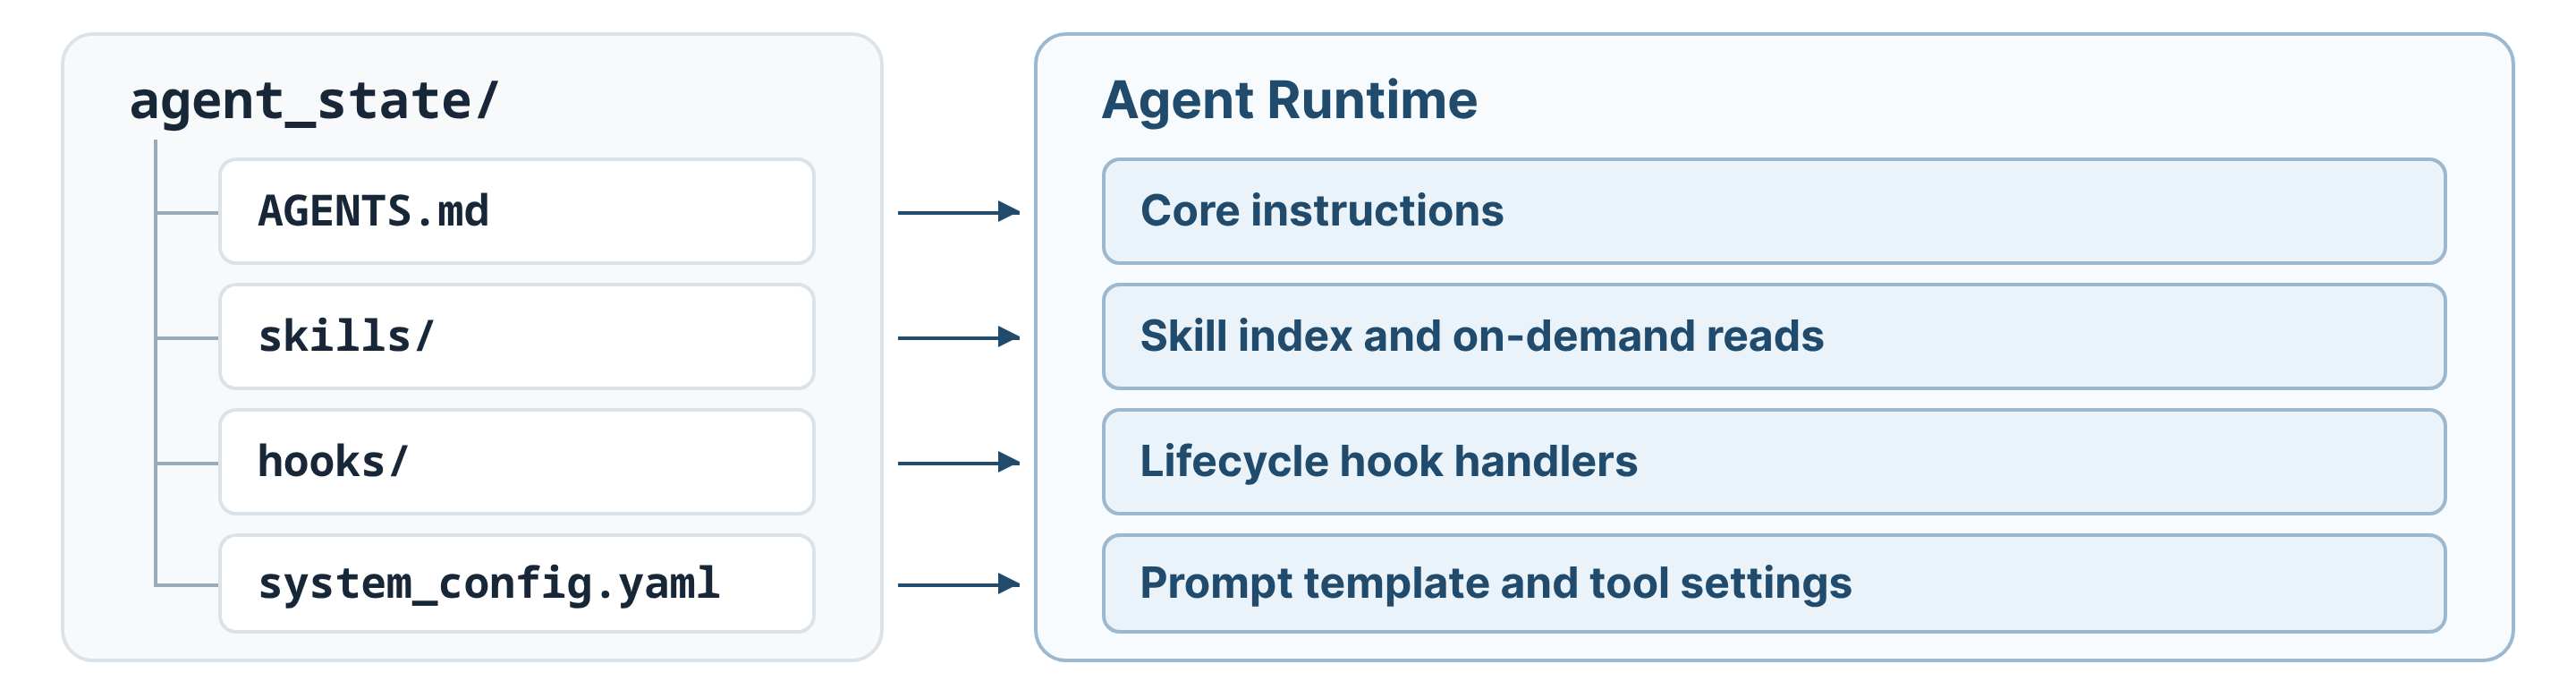
\includegraphics[width=\textwidth]{figs/figure-2-file-centric-architecture.png}
  \caption{The file-centric architecture of \fwname. Agent instructions, skills, hooks, and runtime configuration are organized in separate files and directories and used by the corresponding parts of the runtime.}
  \label{fig:file-centric}
\end{figure*}

\paragraph{State as files.}
\fwname represents mutable agent state as ordinary files, including core instructions, modular skills, lifecycle hook scripts, and runtime configuration (Figure~\ref{fig:file-centric}). An optimizer can edit one instruction or skill locally through the same file operations available to the agent. This gives RSI methods a direct interface to the agent state.

\paragraph{Minimal tools and a portable protocol.}
Tool names, descriptions, and parameter schemas recur in model requests. Large sets of specialized tools increase their fixed token cost and expand the choices the model has to consider. \fwname provides core primitives for file reading, writing, and editing, terminal execution and interaction, and subagent delegation. It uses a short default system prompt and avoids attaching a changing environment snapshot to each user message. The same file-based agent state can run with different cloud or local models through the harness.

\subsection{Evolution and Runtime Cost: On-Demand Context and Lifecycle Prompt Caching}
\label{sec:prompt-cache}

The inference cost of long sessions and repeated RSI experiments depends on both the amount of context sent on each turn and the fraction of prompt tokens that can be read from cache. Context includes the system prompt, tool definitions, and accumulated history. Model providers can charge a lower rate for reading a cached prefix that matches the current request. \fwname limits the context sent to the model and reuses request prefixes across the session lifecycle.

\paragraph{On-demand context loading.}
The system prompt includes only the name and a short trigger description for each installed skill. The agent reads a skill's full instructions from disk when it needs them.

The harness also caps the text returned to the context by a single tool call at 16,000 characters by default. For a long command output, it retains the beginning and end, the exit code, and the path to the complete output on disk. The agent can recover intervening details through file reads or search.

\paragraph{Prompt caching across the session lifecycle.}
At the start of each context segment, \fwname assembles the system prompt and tool definitions. Subsequent turns append messages to the history. Changes written to the agent's files during a segment are loaded at the start of the next segment. When the context reaches its compaction threshold, the summary request reuses the current system prompt, tools, and history and appends a summarization instruction. The next segment loads the updated state and continues from the summary.

\begin{figure*}[t]
  \centering
  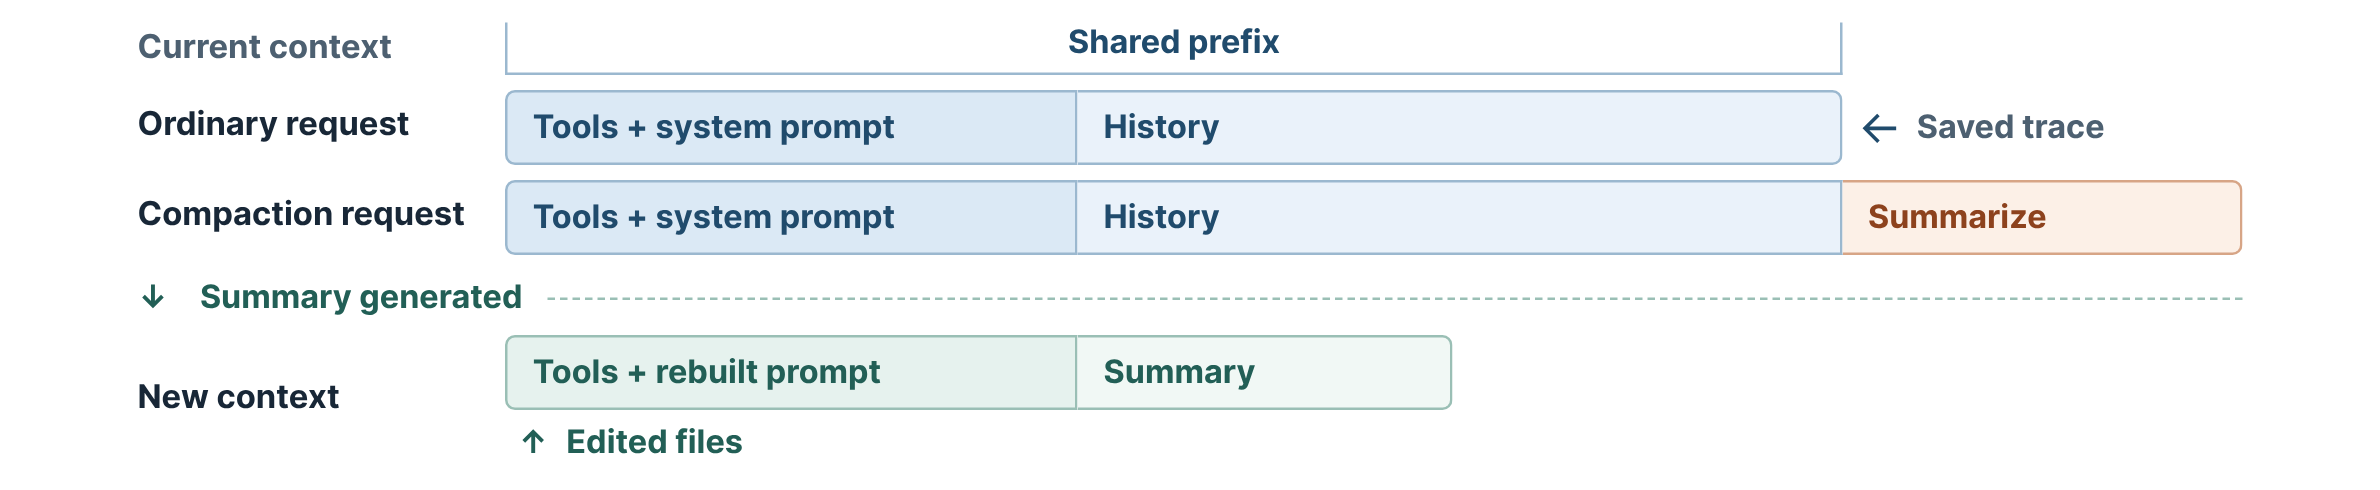
\includegraphics[width=\textwidth]{figs/figure-3-prompt-cache-reuse.png}
  \caption{Prompt-cache reuse across the session lifecycle. A compaction request appends a summarization instruction to the existing prefix. On resumption, the engine replays the system prompt and history from the trace. A new context loads the current file state and continues from the summary.}
  \label{fig:prompt-cache}
\end{figure*}

When resuming a session with an open context, the engine restores the original system prompt and committed history from the trace, preserves model reasoning signatures, and replays tool outputs in their original order. After an interruption, new input is appended to the committed history. Figure~\ref{fig:prompt-cache} illustrates compaction and resumption.

Continuous integration checks the requests produced by the engine with an offline prompt-cache simulator across session-lifecycle scenarios.

\subsection{Pluggable Plugin System}
\label{sec:plugins}

During self-improvement, agents may install, remove, or update tools and workspace plugins in addition to changing instructions and skills. \fwname supports these operations through a pluggable system. We model the lifecycle of its core modules in Lean~4 and prove three properties of the model.

\begin{enumerate}
  \item \textbf{Installation-order independence.} Permuting the installation order yields the same harness state for a given set of enabled plugins.
  \item \textbf{Clean removal and failure isolation.} Installing and then removing a plugin restores the modeled state. If a plugin fails to start and is skipped, the resulting state is equivalent to starting with only the usable plugins.
  \item \textbf{Exclusive state transfer during hot reload.} Live state transfers to the new instance without simultaneous ownership by the old and new instances, avoiding conflicting use or release of that state.
\end{enumerate}

These properties address state accumulation across repeated installation and removal, failure handling during startup, and state ownership during updates. Keeping plugin lifecycle changes predictable supports repeated RSI experiments in a common execution environment.
